\minitoc

\vfill

In this appendix, are presented notions from statistical learning were useful in this work.
This constitutes a simple reminder and is not a thorough survey of the field.

First, in Section~\ref{sec::classifiers::notations}, we present the notations used in this chapter.
Next, Section~\ref{sec::classifiers::svm} presents details about the inner workings of the \gls{acr::svm} algorithm.
Third and last, \glspl{acr::rf} are presented in Section~\ref{sec::classifiers::rf}.

\clearpage

\section{Notations}
    \label{sec::classifiers::notations}
    In this subsection, we denote a family of \(n\) observations and their classes by
    \begin{equation*}
        \left(O^i, y^i\right)_{i = 1, 2, \dots, n}.
    \end{equation*}
    One way of representing an observation \(O\) is to compute a number \(d \in \mathbb{N}^*\) of features (or attributes):
    \begin{equation*}
        \forall j = 1, 2, \dots, d \;, x_j \in \mathscr{X}_j
    \end{equation*}
    These coefficients are aggregated to form a feature vector 
    \begin{equation*}
        \bm{x} \triangleq \left(x_1, x_2, \dots, x_d\right) \in \prod_{i=1}^{d} \mathscr{X}_j
    \end{equation*}
    that corresponds to the observation \(O\).
    Such a mapping \(O \mapsto \bm{x}\) is called a feature map.
    A special case is when \(\forall j=1, 2, \dots, d\;, \mathscr{X}_j = \mathbb{R}\) and feature vectors are Euclidean ones.
    \begin{equation*}
        \forall i = 1, 2, \dots, n \;, \bm{x^i} \in \mathbb{R}^d.
    \end{equation*}
    In practice, observations are often confused with fetaure vectors.

    Classes are modeled by a finite set bijective to the set \(\left\{1, 2, \dots, C\right\}\):
    \begin{equation*}
        \forall i = 1, 2, \dots, n \;, y_i \in \left\{1, 2, \dots, C\right\}.        
    \end{equation*}
    The goal in supervised classification is to learn, based on the training set \(\left(\bm{x^i}, y^i\right)_{i = 1, 2, \dots, n}\), some statistical characteristics in order to predict the classes of some new observations:\footnote{This family is usually called the test set.}
    \begin{equation*}
        \left(\bm{x^i}\right)_{i=n + 1, n + 2, \dots, n + n'}.
    \end{equation*}
    This type of problems is said to be multi-class: each instance has one possible class out of a number of possibilities.
    In the special case of binary classification, only two classes are possible:
    \begin{equation*}
        \forall i = 1, 2, \dots, n \;, y^i \in \left\{0, 1\right\}
    \end{equation*}

    On another hand, the multi-label classification problem is the case where to each instance corresponds a number $L$ of binary labels:
    \begin{equation*}
        \forall i = 1, 2, \dots, n \;, y^i = (y^i_1, y^i_2, \dots, y^i_L) \in \left\{0, 1\right\}^L.
    \end{equation*}
    In this case, associating features with each label \(\left(\bm{x^i}, y^i_l\right)_{i = 1, 2, \dots, n}\) can be seen as an independent binary classification problem.
    This is different from multi-class problems, as for the latter only one class is possible while in the other multiple labels can be detected per instance.\\

    Hereafter, are presented the two supervised classifiers that were used in this work.

\section{\acrlong*{acr::svm}}
    \label{sec::classifiers::svm}
    \glspl{acr::svm} are a special type of linear classifiers.
    The initial classes $\left(y^k\right)_{k=1, 2, \dots, n}$ are transformed into $\left(\tilde{y}^k\right)_{k=1, 2, \dots, n}$ using the map: $y \mapsto \tilde{y} = 2\cdot y - 1$.
    There are always two possible classes $\left\{1, -1\right\}$.
    This simple transformation is use so as to simplify the latter equations.

    We remind the reader of the decision function\footnote{A decision function assigns a class to given observation.} of a linear classifier:
    \begin{equation}
        \label{eq::linear}
        \begin{aligned}
            \mathbf{D}_{\text{linear}, \bm{w}, b}: \mathbb{R}^d &\rightarrow \left\{-1, 1\right\}\\
            \bm{x} &\mapsto 2 \cdot \mathbb{1}_{\bm{w}^\intercal \cdot \bm{x} + b\geq 0} - 1 \quad.
        \end{aligned}
    \end{equation}
    where:
    \begin{conditions}
        \bm{w} & is the weight vector;\\
        b & is the bias.
    \end{conditions}

    \subsection{Hard margin}
        In order to understand the idea behind the \gls{acr::svm} classifier, we start by assuming that the dataset to be classified $\left((\bm{x}^k, y^k)\right)_{k=1, 2, \dots, n}$ is linearly separable.
        It means that there is at least one hyperplane $(H_0)$ that can separate perfectly the two classes.
        We can order points of one class based on their distance to the hyperplane $(H_0)$: $\bm{x} \mapsto d(\bm{x}, H_0)$.
        The closest positive (\textit{resp.} negative) points (i.e., of class $1$ (\textit{resp.}  $-1$)) to $(H_0)$ are called positive (\textit{resp.} negative) support vectors.
        Support hyperplanes are the hyperplanes that are parallel to the separator and pass through the support vectors.
        This can be summarized as:
        \begin{eqnarray}
            \left\{\bm{x}^+_s: s = 1, 2, \dots, n_{psp}\right\} &\triangleq \arg\min\left\{d(\bm{x}_k, H_0) : k=1, 2, \dots, n \wedge \tilde{y}^k = 1\right\}\\
            \left\{\bm{x}^-_s: s = 1, 2, \dots, n_{nsp}\right\} &\triangleq \arg\min\left\{d(\bm{x}_k, H_0) : k=1, 2, \dots, n \wedge \tilde{y}^k = -1\right\}
        \end{eqnarray}
        where:
        \begin{conditions}
            n_{psp} & is the number of positive support vectors.\\
            n_{nsp} & is the number of negative support vectors.\\
        \end{conditions}

        We define:
        \begin{equation*}
            Sol \triangleq \left\{\omega \in \mathbb{R}^d : \omega.\bm{x} + b = 0\right\}.
        \end{equation*}
        We verify that:
        \begin{equation*}
            \forall \lambda \in \mathbb{R}^*, \; (\bm{w}, b) \in  Sol \Leftrightarrow (\lambda . \bm{w}, \lambda.b) \in Sol.
        \end{equation*}
        In other words, the solution $(\bm{w}^*, b^*)$ is unique up to multiplicative term $\lambda \in \mathbb{R}^*$.
        In this context, $(\bm{w}, b)$ is chosen so that \(\bm{w}\) points to the positive instances\footnote{The positive instances are inside the positive half-space.} and the support hyperplanes verify:
        \begin{equation}
            \label{eq::support_lines}
            \begin{cases}
                \forall s = 1, 2, \dots, n_{psp} \quad \bm{w}^\intercal\cdot\bm{x}^+_s + b = 1\\              
                \forall s = 1, 2, \dots, n_{nsp} \quad \bm{w}^\intercal\cdot\bm{x}^-_s + b = -1                
            \end{cases}
        \end{equation}

        \begin{figure}
            \centering
            \includestandalone[mode=buildmissing, width=.7\textwidth]{figures/svm/linear_separable}
            \caption[
                Illustration of the hard-margin \acrshort*{acr::svm}.
            ]{
                \label{fig::linear_separable} 
                Illustration of the hard-margin \gls{acr::svm}.
                A hyperplane separator in $\mathbb{R}^2$ corresponds to a line.
                In this case, $n_{psp} = n_{nsp} = 1$.
                The support lines are plotted in orange.
                $M$ is the margin.
            }
        \end{figure}

        Figure~\ref{fig::linear_separable} illustrates these notions.
        The uncertainty of a point classification is an increasing function of the distance of that point to the separator.
        In the hard margin case, the given samples are supposed to be certain.
        Since support vectors are the closest certain points to $(H_0)$, the class of points $\bm{p}$ that verify $\vert\bm{w}^\intercal\cdot\bm{p} + b\vert \geq 1$ is known with probability $1$.
        Conversely, the points that lie between the support hyperplanes are the most uncertain.
        The bigger the distance between these two lines, the more nuanced the classifier decision is.
        The main idea behind \glspl{acr::svm} is to maximize this distance.
        It is called margin and denoted by $M$.\\

        In order to compute the margin, we can interpret it as the length of the orthogonal projection of any vector $\bm{v}_{st}$\footnote{$\forall (s, t) \in \left\{1, 2, \dots, n_{nsp}\right\} \times \left\{1, 2, \dots, n_{psp}\right\}$.} going from a negative support vector $\bm{x}^-_s$ to a positive one $\bm{x}^+_t$ on any line carried by $\bm{w}$.
        Since all support vectors of the same class lay on the same line, the choice of $(s,t)$ is inconsequential.
        We can hence deduce:
        \begin{align}
            M &= \frac{\bm{w}^\intercal}{\Vert\bm{w}\Vert} \cdot (\bm{x}^+_1 - \bm{x}^-_1) \nonumber \\
            M &= \frac{2}{\Vert\bm{w}\Vert}
        \end{align}

        Maximizing $M$ is actually equivalent to minimizing $\Vert\bm{w}\Vert$.
        In the purpose of simplifying the resolution of the problem, we drop the square root and minimize instead $\Vert\bm{w}\Vert^2$.
        The certainty in the given samples is translated by the inequalities:
        \begin{equation*}
            \begin{cases}
                \bm{w}^\intercal\cdot\bm{x}^i + b \geq 1 & \forall i \in \left\{1, 2, \dots, n: \tilde{y}^i = 1\right\}\\
                \bm{w}^\intercal\cdot\bm{x}^i + b \leq -1 & \forall i \in \left\{1, 2, \dots, n: \tilde{y}^i = -1\right\}
            \end{cases}.
        \end{equation*}
        These can be summed in one, as follows:
        \begin{equation}
            \label{eq::hard_margin}
            \tilde{y}^i.(\bm{w}^\intercal\cdot\bm{x}^i + b) \geq 1 \; \forall i = 1, 2, \dots, n.
        \end{equation}
        Thus, the \gls{acr::svm} problem can be formalized as a convex constrained quadratic optimization one:
        \begin{equation}
            \label{eq::hard_svm_primal}
            \begin{aligned}
                & \min_{\bm{w}}
                & & {\Vert \bm{w} \Vert}^2 \\
                & \text{s.t.}
                & & \tilde{y}^i.(\bm{w}^\intercal\cdot\bm{x}^i + b) \geq 1 \; \forall i = 1, 2, \dots, n
            \end{aligned}.
        \end{equation}

    \subsection{Soft margin}
        In the previous case, we assumed that we are always certain about the classes of the given samples.
        The margin cannot contain any of those points.
        This explains the name hard margin.
        We are always guaranteed to have a solution of a hard margin \gls{acr::svm} in the case of linear separability.
        However, if the last condition is not met, there is no such solution.
        To alleviate this problem,~\textcite{cortes1995support} allowed some uncertainty in the given samples in order to fit the linear model.\\

        \begin{figure}
            \centering
            \includestandalone[mode=buildmissing, width=.7\textwidth]{figures/svm/non_linear_separable}
            \caption[
                Illustration of a soft margin \acrshort*{acr::svm}.
            ]{
                \label{fig::soft_margin} Illustration of a soft margin \gls{acr::svm}.
                The orange lines (\textit{resp.} green line) correspond to the support hyperplanes (\textit{resp.} separator).
                Dataset points are allowed to be inside the margin and even in the other side of the separator.
                It helps fit a natively linear classifier in a non linearly separable case.
            }
        \end{figure}

        To put this into mathematical terms, we start by the reminding the constraint of the hard margin problem in Equation~\ref{eq::hard_margin}.
        Allowing uncertainty for some given point $\bm{x}^i$ comes back to allowing it to be in the wrong side of the support hyperplane: i.e., $\tilde{y}^l.(\bm{w}^\intercal\cdot\bm{x}^l + b) < 1$.
        In this case, we define: $\xi^i := 1 - \tilde{y}^i.(\bm{w}^\intercal\cdot\bm{x}^i + b) > 0$.
        Otherwise, $\xi^i := 0$.
        These defined values are called slack variables.
        They express how much each point is uncertain.
        They can be expressed in a compressed form called hinge loss:
        \begin{equation}
            \label{eq::slack_variables}
            \xi^i \triangleq \max\left(1 - \tilde{y}^i.(\bm{w}^\intercal\cdot\bm{x}^i + b), 0\right).
        \end{equation}
        The soft margin constraint translates now to:
        \begin{equation}
            \label{eq::soft_margin}
            \tilde{y}^i.(\bm{w}^\intercal\cdot\bm{x}^i + b) \geq 1 - \xi^i.
        \end{equation}
        Four cases can be distinguished for slack variables:
        \begin{itemize}[label=\(\blacktriangleright\)]
            \item \(\xi^i = 0\): the class of the point is certain;
            \item \(0 < \xi^i \leq 1\): the point is of the same class but is uncertain: i.e., between the support hyperplane and the separator;
            \item \(1 < \xi^i < 2\): the point is of the opposite class and is uncertain: i.e., between the separator and the opposite support hyperplane;
            \item \(2 \leq \xi^i\): the point is certainly of the opposite class: i.e., beyond the opposite support hyperplane.
        \end{itemize}
        As a consequence, when a dataset is not linearly separable, at least one sample $i_0$ cannot fit in a linear model and $1 < \xi^{i_0}$.
        All these situations are illustrated in Figure~\ref{fig::soft_margin}.\\

        The idea is to find a configuration where most slack variables are null or near $0$.
        Sparsity is also required: we prefer having one wrong point rather than a lot of points that are uncertain.
        For this purpose, these variables would be penalized against using an $L_1$ norm.
        Since all slack variables are positive, the soft margin \gls{acr::svm} problem becomes:
        \begin{equation}
            \label{eq::soft_svm_primal}
            \begin{aligned}
                & \min_{\bm{w} \in \mathbb{R}^d}
                & & {\Vert \bm{w} \Vert}^2 + C \cdot \sum_{i=1}^n \xi^i \\
                & \text{s.t.} & & \tilde{y}^i.(\bm{w}^\intercal\cdot\bm{x}^i + b) \geq 1 - \xi^i, \; \forall i = 1, 2, \dots, n\\
                & & & \xi^i \geq 0, \; \forall i = 1, 2, \dots, n
            \end{aligned}.
        \end{equation}
        where:
        \begin{conditions}
            C & is the penalization constant.\\
        \end{conditions}

        A small value of $C$ means the slack variables are allowed to get big: the margin is expected to be big.
        A high value of $C$ leads to a tight margin as it penalizes any uncertainty.
        The special case where $C=\infty$ corresponds simply to the hard margin case.
        Hence, the penalization constant is tuned, using cross-validation for instance, so as to achieve the best generalization power.

        Since the problem stated in Equation~\ref{eq::soft_svm_primal} is a convex optimization problem, solving it is equivalent to solving the dual:
        \begin{equation}
            \label{eq::soft_svm_dual}
            \begin{aligned}
                & \max_{\alpha_1, \alpha_2, \dots, \alpha_n \in \mathbb{R}_+}
                & & \sum_{1\leq i \leq n} \alpha_i - \frac{1}{2}\cdot\sum_{\substack{1\leq l \leq n\\1\leq p \leq n}}\alpha_l\cdot\alpha_p\cdot\tilde{y}^l\cdot\tilde{y}^p\cdot(\bm{x}^l)^\intercal\cdot\bm{x}^p\\
                &\text{s.t.} & & \sum_{1 \leq i \leq n}\tilde{y}^i\cdot\alpha_i=0 \\
                & & & 0 \leq \alpha_i \leq C \;\forall i = 1, 2, \dots, n
                \end{aligned}
        \end{equation}
        where:
        \begin{conditions}
            \alpha_i & is the Lagrange multiplier corresponding to \(i\)\textsuperscript{th} observation.\\
        \end{conditions}

        A fast solution of this problem is possible using the \gls{acr::smo} developed by~\textcite{platt1998sequential}.
        This will not be detailed herein. 

    \subsection{Kernel \acrshort*{acr::svm}}
        Not all classification problems can be solved in a linear manner.
        Unfortunately, \gls{acr::svm} is inherently linear.
        However, there is a way to generalize this classifier.\\

        \begin{figure}
            \centering
            \ffigbox[\textwidth]{
                \begin{subfloatrow}[2]
                    \ffigbox[\textwidth]{
                        \includestandalone[mode=buildmissing, width=.45\textwidth]{figures/svm/circles_original}
                    }{
                        \caption{
                            \label{subfig::original_circles}
                            Original representation of the dataset in the feature space.
                        }
                    }
                    \ffigbox[\textwidth]{
                        \includestandalone[mode=buildmissing, width=.45\textwidth]{figures/svm/circles_polar}
                    }{
                        \caption{
                            \label{subfig::polar_circles}
                            Representation of the dataset using polar coordinates
                        }
                    }
                \end{subfloatrow}
            }{
                \caption{
                    \label{fig::circles_transformation}
                    Example of a transformation of a dataset that can be linearly separable in the maped space. 
                }
            }
        \end{figure}

        The original feature space where the data is represented is not always an ideal\footnote{An ideal space is one where distances between points are meaningful.} one.
        A solution is to find a transformation $\Phi: \mathbb{R}^d \rightarrow \mathscr{H}$ that maps initial feature vectors into a Hilbert space $(\mathscr{H}, \langle\cdot{,}\cdot\rangle_{\mathscr{H}})$ where distances between instances are meaningful.
        There is no unique map that satisfy this type of properties.
        We are particularly interested in a map which transforms the data into a space where they are hopefully linearly separable~\parencite{boser1992training}.
        This illustrated in Figure~\ref{fig::circles_transformation}.
        Using a polar coordinate transformation 
        \begin{align*}
            \Phi: \mathbb{R}^2 &\rightarrow \mathbb{R}^2 \\
            \begin{bmatrix}
                x \\
                y
            \end{bmatrix} &\mapsto \begin{bmatrix}
                \sqrt{x^2 + y^2} \\
                \operatorname{arctan}_2(y, x)
            \end{bmatrix},
        \end{align*}
        the dataset can be linearly separable.
        In this particular case, the original probability distribution is known as it was generated manually.
        Moreover, the map codomain is a vector space of the same dimension as the map domain.
        This is usually not the case: in practice, the right mapping is difficult to come by\footnote{If it exists at all.} and the codomain is usually of a higher dimension, possibly infinite.
        Finding such a map involves usually heavy computations.
        However, as we are interested in distances between dataset points, there is an easier way around.
        Using the ``kernel trick'', one can compute any distance in the target space $\mathscr{H}$ using only the scalar product:
        \begin{align}
            \label{eq::kernel_definition}
            k: \mathbb{R}^d \times \mathbb{R}^d &\rightarrow \mathbb{R}\\
            (\bm{x}, \bm{y}) &\mapsto \langle\Phi(\bm{x}), \Phi(\bm{y})\rangle_{\mathscr{H}} \nonumber.
        \end{align}
        Going back to the dual optimization problem stated in Equation~\ref{eq::soft_svm_dual}, we see that only the scalar product between samples is needed.
        Assuming the existence of an adequate mapping $\Phi$, and if we substitute each point by its representation in the new space, we can rewrite, so called, kernel \gls{acr::svm}.
        \begin{equation}
            \label{eq::kernel_soft_svm_dual}
            \begin{aligned}
                & \max_{\alpha_1, \alpha_2, \dots, \alpha_n \in \mathbb{R}_+}
                & & \sum_{1 \leq i \leq n} \alpha_i - \frac{1}{2}\cdot\sum_{\substack{1\leq l \geq n\\1\leq p \geq n}}\alpha_l\cdot\alpha_p\cdot\tilde{y}^l\cdot\tilde{y}^p\cdot k(\bm{x}^l, \bm{x}^p)\\
                &\text{s.t.} & & \sum_{1 \leq i \leq n}\tilde{y}^i\cdot\alpha_i=0 \\
                & & & 0 \leq \alpha_i \leq C \; \forall i = 1, 2, \dots, n
                \end{aligned}
        \end{equation}

        There are more theoretical details for kernels which are not discussed herein.
        For more details on the subject, one can check the work by~\textcite{aronszajn1950theory,shawe2004kernel,vapnik2013nature}.

        \subsubsection{Usual kernels.}
            The choice of kernels is not easy.
            Practitioners experiment with different kernel types and parameters.
            One can engineer a kernel specific for their application.
            However, in general, there are some kernels that are frequently chosen:
            \begin{itemize}
                \item the native linear kernel:
                \begin{equation}
                    \label{eq::linear_kernel}
                    k(\bm{x}, \bm{y}) = \bm{x}^\intercal \cdot \bm{y};
                \end{equation}
                \item the \gls{acr::rbf} kernel: for some parameter $(\gamma) \in \mathbb{R}$
                \begin{equation}
                    \label{eq::rbf_kernel}
                    k_{\gamma}(\bm{x}, \bm{y}) = \exp\left(-\gamma \cdot \left\lVert \bm{x} - \bm{y} \right\rVert^2\right);
                \end{equation}
                \item the polynomial kernel: for some parameters $(c, d) \in \mathbb{R}_+ \times \mathbb{N} \setminus \left\{0\right\} $
                \begin{equation}
                    \label{eq::polynomial_kernel}
                    k_{\gamma, c}(\bm{x}, \bm{y}) = (\bm{x}^\intercal \cdot \bm{y} + c)^d;
                \end{equation}
                \item the sigmoid kernel: for some parameters $(\gamma, c) \in \mathbb{R}^2$
                \begin{equation}
                    \label{eq::sigmoid_kernel}
                    k_{\gamma, c}(\bm{x}, \bm{y}) = \gamma \cdot \tanh(\bm{x}^\intercal \cdot \bm{y} + c).
                \end{equation}
            \end{itemize}
            The choice of kernel parameters in important not only for achieving good classification results but also to avoid overfitting problems.

        \subsubsection{\acrlong*{acr::mkl}.}
            Some operations over kernels always yield valid kernels.
            This is true for instance for summation.
            In fact, fixing the number of kernels $K\in \mathbb{N} \setminus \left\{0\right\}$, for basis kernels $k_i \; \forall i = 1, 2, \dots, K$ weigthed by $\mu_i \in \mathbb{R}_+\; \forall i = 1, 2, \dots, K$,
            \begin{equation}
                \label{eq::mkl}
                k(\bm{x}, \bm{y}) = \sum_{i=1}^K \mu_i \cdot k_i(\bm{x}, \bm{y})
            \end{equation}
            is also a valid kernel.
            Such kernels proved to be better in practice than using single kernels~\parencite{lanckriet2004statistical}.
            To simplify the problem, the solution is chosen in the simplex of the basis kernels: i.e., $ (\mu_1, \mu_2, \dots, \mu_K) \in (\mathbb{R}_+)^K  \; s.t. \sum_{i=1}^K \mu_i = 1$.
            Multiple schemes were presented in order to solve the \gls{acr::mkl} \gls{acr::svm} problem~\parencite{rakotomamonjy2008simplemkl,varma2009more,sun2010multiple}.
            
    \subsection{Properties}
        Herein are presented properties of the \gls{acr::svm} classifier based on a practical point of view.
        We start by stating some of its advantages:
        \begin{itemize}
            \item Mathematically guaranteed solution: the convex formulation of the problem implies the existence of a global optimum that can be computed efficiently.
            \item The \gls{acr::smo} can be adapted to an online setting~\parencite{bordes2005fast}.
            \item The soft margin \gls{acr::svm}, with a right tuning of the slackness parameter $C$, can achieve a good generalization.
            \item The \gls{acr::svm} is inherently sparse in the sense that it relies only on a small subset of the data which are support vectors.
                    This implies that with a right kernel the \gls{acr::svm} can handle imbalanced datasets.
        \end{itemize}
        On the other hand it suffers also from some drawbacks, listed hereafter:
        \begin{itemize}
            \item Finding a the right kernel to represent that data is not a simple task.
                    Even with an expert knowledge, one can easily overfit to the training data.
            \item In the same sense, parameter fitting is not straight-forward and time-consuming.
                    Practically, it is a result of a trial and error or grid search approach.
            \item Eventhough it can be adapted to multi-class or multi-output settings, the \gls{acr::svm} is natively designed for binary classification.
            \item \gls{acr::svm} does not handle well attributes of different types.
                    Feature vectors are preprocessed, usually normalized, before training.
            \item \gls{acr::svm} does not yield probabilities natively.
                    Although it is possible to compute scores that are in the unit interval, these are difficult to interpret as probabilities.
        \end{itemize}

\section{\acrlong*{acr::rf}}
    \label{sec::classifiers::rf}
    A \gls{acr::rf} is an agregation of decision tree classifiers.
    First, is explained how the latter works.
    Afterwards, we describe how the aggregation of basic classifiers can be beneficial for classification, especially in the case of decision trees.
    We end this Section discussing some \gls{acr::rf} properties.

    \subsection{Decision tree classifier}
        \begin{figure}[htb]
            \centering
            \includestandalone[mode=buildmissing, width=\textwidth]{figures/random_forest/decision_tree}
            \caption[
                A visualization of a decision tree classifier learned using $I_G$ Gini index over the iris dataset.
            ]{
                \label{fig::decision_tree_graph}
                A visualization of a decision tree classifier learned using $I_G$ Gini index over the iris dataset~\parencite{fisher1936use}.
                Three classes are possible.
                Each non leaf node states a thresholding condition.
                For a leaf, its class is presented instead.
                ``dist.''stands for distribution of classes in each node.
                The whole decision tree overfits to the data with a \SI{100}{\percent} overall accuracy ratio.
                However, when cut at depth 2, the overall accuracy ratio does not drop noticeably (\SI{96}{\percent}).
            }
        \end{figure}

        The decision tree classifier consists in successive conditions.
        It is easily modeled as a tree graph rooted at $r$.
        Each non leaf node $b$ in tree takes as input an observation $\bm{x}$ which is fed to logical predicate $P_b$\footnote{$P_b(\bm{x})$ can takle only two values.}: exactly two children are possible per node.
        These predicates are of a specific form: only one dimension $i_b$ of the data is taken into account.
        The output is then computed by applying a threshold $t_b$ to $x_{i_b}$.
        This can be simplified as $P_b(\bm{x}) = \mathbb{1}_{x_{i_b} \geq t_b} $.
        The chosen child is denoted $d_b(\bm{x}) \leftarrow \operatorname{child}(b, \mathbb{1}_{x_{i_b} \geq t_b})$.
        Leafs are the terminal nodes of the tree and they do not apply any predicate to their input.
        Instead, based on the assigned class $c(l) \in \left\{1, 2, \dots, C\right\}$ of the leaf $l$, they predict the label of the input.
        Each dimension $x_i \in \mathscr{X}_i$ is treated separately.
        Hence, decision trees can handle heterogenous feature vectors that are no longer restricted to be $\mathbb{R}^d$.
        The decision function of a decision tree classifier can be written as:
        \begin{equation}
            \label{eq::df_decision_tree}
            \begin{aligned}
                D_{\text{decision tree}}: \prod_{i=1}^{d}\mathscr{X}_i &\rightarrow \left\{1, 2, \dots, C\right\}\\
                \bm{x} &\mapsto c\left(d_{d_{\ddots_{d_r(\bm{x})}}(\bm{x})}\right)
            \end{aligned}
        \end{equation}
        This representation is complicated and too abstract and is never used.
        The intuitive representation of decision tree classifiers, shown in Figure~\ref{fig::decision_tree_graph}, is generaly prefered.
        In Figure~\ref{fig::decision_tree_separator}, we can clearly attribute the fact that the separator is an aggregation of vertical and horiontal segments to the fact that only one dimension is taken into acount at a time.\\

        \begin{figure}[htb]
            \centering
            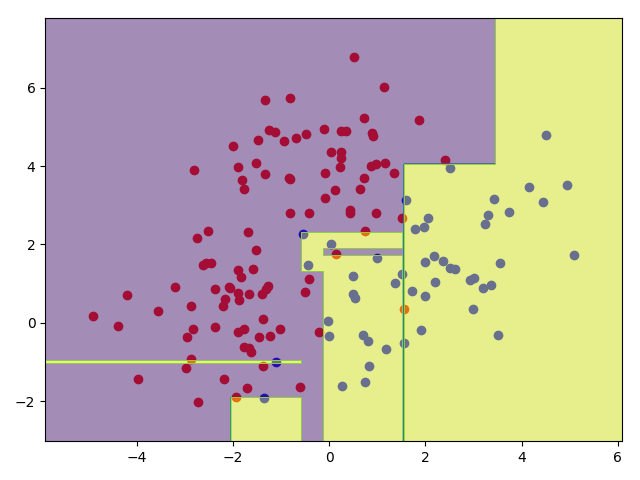
\includegraphics[width=.5\textwidth]{images/related_work/decision_tree_separator}
            \caption[
                Visualization of a decision tree separator trained over generated data in a two dimensional feature space.
            ]{
                \label{fig::decision_tree_separator}
                Visualization of a decision tree separator trained over generated data in a two dimensional feature space.
                The separator is composed exclusively of horizontal and vertical lines.
                We can also see how the decision tree overfits by adding narrow splits to accomodate lone points surrounded by others with an opposite class.
            }
        \end{figure}

        Up to now, we assumed the decision tree to be already in place.
        The training step of this supervised classifier consists in determining its structure and all the thresholds.
        The goal is to have leafs with no prediction errors.
        In other words, all observations that end up in a leaf must be of the same class: the leaf is called pure.
        Consequently, to each node that is not pure would be associated a predicate that would hopefully distinguish amongst incoming observations.
        This is done recursively starting from the root.\\

        The choice of the splitting dimension and the threshold at each node is made in the aim of achieving the most gain in the ``purity'' of child nodes.
        As a consequence, there is a need of a metric $I$ that can describe the heterogeneity, as the opposite of purity, of a node.
        These are usually based on a probabilistic interpretation as they compute the fraction of observations $p_c$ that go through a node of class $c \in \left\{1, 2, \dots, C\right\}$.
        Three examples are provided:
        \begin{description}
            \item[Gini index:]
            \begin{equation}
                \label{eq::gini}
                I_G\left(\left(p_c\right)_{c=1, 2, \dots, C}\right) = \sum_{c=1}^{C} p_c \cdot \sum_{\substack{l=1, 2, \dots, C\\l \neq c}} p_l;
            \end{equation}
            \item[Entropy:]
            \begin{equation}
                \label{eq::entropy}
                I_H\left(\left(p_c\right)_{c=1, 2, \dots, C}\right) = - \sum_{c=1}^{C} p_c \cdot \log_2(p_c);
            \end{equation}
            \item[Variance:]
            \begin{equation}
                \label{eq::variance_index}
                I_V\left(\left(x_{d_s}^i\right)_{i\in S}\right) = \frac{1}{2 \cdot \vert S \vert^2} \cdot \sum_{(i,j) \in S\times S} \left(x_{d_s}^i - x_{d_s}^j\right),
            \end{equation}
            where:
            \begin{conditions}
                d_s & is the chosen dimension to split over;\\
                S & $\subset \left\{1, 2, \dots, n\right\}$ is an set of indices.
            \end{conditions}
        \end{description}
        Considering $S_b$ the set of indices of inputs going through a node $b$, one can compute the gain of a split at node $b$ as:
        \begin{equation}
            \label{eq::split_gain}
            G_b \triangleq I(S_b) - \sum_{c \in \left\{d_b(\bm{x}^i): i \in S_b\right\}} I(S_c)
        \end{equation}
        The optimal splitting dimension and threshold are chosen so that they maximizes the gain $G_b$.
        Details of how this is computed is outside ths scope of this manuscript and is not provided herein.
        For more information on the subject the reader may refer to the work of~\textcite{breiman1984classification}.\\

        Stopping only when total purity is achieved can yield complicated decision trees that overfit easily.
        This motivates the use for some early stopping criteria:
        \begin{itemize}
            \item a minimal number of observations going through each node.
            \item a minimal purity ratio computed as the ratio of all instances going through the node having the dominant class.
            \item a maximal depth of the tree.
        \end{itemize}
        To conclude, the class at each leaf is taken as the dominant class of instances entering it.

    \subsection{Bagging decision trees}
        \begin{figure}
            \centering
            \includestandalone[mode=buildmissing, height=.4\textheight]{figures/random_forest/ensemble}
            \caption[
                Illustration of the principle of ensemble methods.
            ]{
                \label{fig::ensemble} Illustration of the principle of ensemble methods.
                For each decision function $\forall l=1,2,3\;D_l$, is represented the set where the each classifier fails $F(D_l) \leftarrow \left\{(\bm{x}, y) \in \prod_{i=1}^{d}\mathscr{X}_i \times \left\{1, 2, \dots, C\right\} : D_l(\bm{x}) \neq y\right\}$.
                In the case of unweigthed bagging, the aggregated classifier will fail when more than half of the classifiers fail.
                In this case, the set $F(D_{\text{bagging}})$ is the union of intersections of two different $F(D_l)$: $F(D_{\text{bagging}}) = \bigcup_{l\neq p} F(D_l) \cap F(D_p)$.
                In this case where classifiers are diverse, the aggregated one fails less frequently than each single one.
            }
        \end{figure}

        \begin{figure}
            \centering
            \ffigbox[\textwidth]{
                \begin{subfloatrow}[2]
                    \ffigbox[\textwidth]{
                        \includestandalone[mode=buildmissing, width=.45\textwidth]{figures/random_forest/circles_dt}
                    }{
                        \caption{
                            \label{subfig::decision_tree_circles} Decision tree separator
                        }
                    }
                    \ffigbox[\textwidth]{
                        \includestandalone[mode=buildmissing, width=.45\textwidth]{figures/random_forest/circles_rf}
                    }{
                        \caption{
                            \label{subfig::rf_circles} \gls{acr::rf} separator (in purple) with constituing decision trees
                        }
                    }
                \end{subfloatrow}
            }{
                \caption[
                    Difference between a single decision tree and an \gls{acr::rf} visualized in feature space for a generated toy data.
                ]{
                    \label{fig::decision_tree_vs_rf}
                    Difference between a single decision tree and an \gls{acr::rf} visualized in feature space for a generated toy data.
                    We see how an \gls{acr::rf} aggregates multiple shallow decision trees in order to achieve a good generalization power instead of overfitting to the sampled data.
                }
            }
        \end{figure}

        While reducing the complexity of the decision tree can help avoid overfitting problems, one can risk, on the other hand, an underfitting in the classification.
        In order to find a compromise, an ensemble method can be adopted.
        The principle of this type of approaches is to multiply different underperforming classifiers and aggregate them together.
        These classifiers should be taken as diverse as possible in order to cover the whole feature space.
        The aggregation is achieved through a majority vote and, if the classifiers can provide probabilities, the vote can be weighted by the latter.
        This is illustrated in Figure~\ref{fig::ensemble}.
        Formally, the decision function of an unweighted aggregation of classifiers $\left(D_l\right)_{l = 1, 2, \dots, L}$ can be written as:
        \begin{equation}
            \label{eq::decision_function_hard_ensemble}
            \begin{aligned}
                D_{\text{hard ensemble}, \left(D_l\right)_{l = 1, 2, \dots, L}}: \prod_{i=1}^{d}\mathscr{X}_i &\rightarrow \left\{1, 2, \dots, C\right\}\\
                \bm{x} &\mapsto \arg \max_{c = 1, 2, \dots, C}\lvert\left\{l\in\left\{1, 2, \dots, L\right\}: D_l(\bm{x}) = c\right\}\rvert
            \end{aligned},
        \end{equation}
        while the weighted aggregation using classifier output probabilities $\left(p_l\right)_{l = 1, 2, \dots, L}$ is expressed as:
        \begin{equation}
            \label{eq::decision_function_weighted_ensemble}
            \begin{aligned}
                D_{\text{weighted ensemble}, \left((D_l, p_l)\right)_{l = 1, 2, \dots, L}}: \prod_{i=1}^{d}\mathscr{X}_i &\rightarrow \left\{1, 2, \dots, C\right\}\\
                \bm{x} &\mapsto \arg \max_{c = 1, 2, \dots, C} \sum_{l=1}^{L} p_l\left(D_l(\bm{x}) = c\right) 
            \end{aligned}.
        \end{equation}

        Bagging is an instance of ensemble approach.
        In order to have different classifiers specializing in a certain pattern, each one is trained on a randomly determined subset of the training data~\parencite{breiman1996bagging}.
        The idea is that each one of these subsets would exhibit a particular aspect that is crucial for the classification.
        The aggregation of each classifier knowledge would eventually help generalize at prediction time.\\

        \gls{acr::rf} do not only rely on a simple bagging but also on a second random sampling: this time it is on the feature dimensions.
        When splitting a node at training time, only a subset of randomly chosen dimensions is considered~\parencite{breiman2001random}.
        We depict in Figure~\ref{fig::decision_tree_vs_rf} the difference between an \gls{acr::rf} and a single decision tree.

    \subsection{Properties}
        \glspl{acr::rf} are often used in practice as they offer some advantages.
        Hereafter are listed some of these:
        \begin{itemize}
            \item As decision trees deal with each feature independently, they can natively, as well as \glspl{acr::rf}, handle heterogenous data.
                It can handle boolean features along with integer or real ones.
            \item Since at each time only a subset of features is considered, \glspl{acr::rf} can scale easily under high dimensionality.
            \item The ensemble character of \glspl{acr::rf} allows them to adapt to outliers and hence, provided a large enough trainning dataset, can achieve a good generalization power.
            \item Prediction relies on simple comparisons and can be computed quickly.
            \item They yield probabilities that are consistent.
            \item They are inherently multi-class and do not need to be adapted.
        \end{itemize}
        As seen with \glspl{acr::svm}, \glspl{acr::rf} have also some issues:
        \begin{itemize}
            \item It is not simple to interpret results of \glspl{acr::rf} and connect specific trees to recognizable patterns.
            \item They can take up a lot of memory to store all trees.
                    They can also require a lot of computations to train.
            \item They do not allow the possibility of using kernels to represent the data.
            \item They do not handle well imbalanced datasets and must be adapted accordingly.
        \end{itemize}

